%  Synergies and mergers-Thursday, 19 November 2020
%
%  Created by Patrick on 2020-11-19.
%  Copyright (c) 2020 __Patrick Legros__. All rights reserved.
%
%!TEX encoding = UTF-8 Unicode  

\documentclass[a4paper,leqno]{article}%leqno to number equations on the left
\usepackage[utf8]{inputenc}
\usepackage{amsthm,amsmath,amssymb,amsfonts}
\usepackage{url}
\usepackage{hyperref}
\usepackage[round]{natbib}
%\bibliographystyle{plainnat}
\usepackage[mathscr]{euscript}
\let\euscr\mathscr \let\mathscr\relax
\usepackage[scr]{rsfso}
\usepackage{graphicx}
\usepackage{float}
\usepackage{enumerate}
\usepackage{blindtext}
\usepackage{setspace}
\usepackage{eurosym}
\usepackage{hyperref}
\usepackage{pdflscape}
\usepackage{array, multirow}
\usepackage[dvipsnames]{xcolor}
\usepackage{enumitem}
\usepackage{todonotes}

\usepackage{tikz}
\hypersetup{
colorlinks,
citecolor=NavyBlue,
linkcolor=NavyBlue,
urlcolor=NavyBlue}
\usetikzlibrary{matrix}
\newtheorem{prop}{Proposition}
\newtheorem{lemma}{Lemma}
\newtheorem{corollary}{Corollary}
\newtheorem{ass}{Assumption}
\newtheorem{result}{Result}
\newtheorem{condition}{Condition}
\newtheorem{Theorem}{Theorem}
\newtheorem{Definition}{Definition}
\newtheorem{remark}{Remark}
\newtheorem{example}{Example}

\newenvironment{reusefigure}[2][htbp]
  {\addtocounter{figure}{-1}%
   \renewcommand{\theHfigure}{dupe-fig}% If you're using hyperref
   \renewcommand{\thefigure}{\ref{#2}}% Figure counter is \ref
   \renewcommand{\addcontentsline}[3]{}% Avoid placing figure in LoF
   \begin{figure}[#1]}
  {\end{figure}}
  
  \usepackage{titlesec}

%\setcounter{secnumdepth}{4}

\titleformat{\paragraph}
{\normalfont\normalsize\bfseries}{\theparagraph}{1em}{}
\titlespacing*{\paragraph}
{0pt}{3.25ex plus 1ex minus .2ex}{1.5ex plus .2ex}

 \usepackage{geometry}

 
 \newcommand{\E}{\mathbb E}
 \newcommand{\N}{\mathcal N}
\renewcommand{\th}{\hat\theta}
\renewcommand{\t}{\theta}
\renewcommand{\a}{\alpha}
\renewcommand{\b}{\beta}
\newcommand{\s}{\sigma}
\newcommand{\de}{\delta}
\newcommand{\uut}{\underline{\underline{\theta}}}
\newcommand{\ut}{\underline{\theta}}
\newcommand{\uv}{\underline{v}}
\newcommand{\ov}{\overline{v}}
\newcommand{\up}{\underline{p}}
\newcommand{\op}{\overline{p}}


\begin{document}


\title{Data Driven Mergers and Synergistic Information}
\author{Antoine Dubus and Patrick Legros\thanks{We would like to thank.}}
\date{\today}

%\author{Antoine Dubus\thanks{~~Université Libre de Bruxelles, ECARES; \href{mailto:antoine1dubus@gmail.com}{antoine1dubus@gmail.com}.}}

\maketitle

 
\textbf{Very preliminary, do not circulate.}

\baselineskip0.7cm
Mergers fail, claimed efficiencies at the time of merger review are often not realized, or if they are realized, they are not passed through to consumers. Is this because firms claim that the merger will yield efficiency gains in the hope of convincing authorities? Is it because firms haven't done the homework and incorrectly evaluated the extent of synergies? Or is it because synergies exist ``on average'' only, hence that there is a probability that ex-post synergies may not exist?

These questions make sense in a world where firms are unsure of the extend of synergies at the time they decide to merge. In such an environment, more precise information about the level of synergies that will follow a merger is valuable not only for the firms but also for the regulator. One way for such an information can be generated is by collaborating in a soft-way in order to learn whether a full merger is beneficial. While there is a value to such information acquisition there are also costs: the information changes the competitive positions of the firms if the merger does not go through, but also changes the desire of a regulator -- who is aware of this information or can infer it from the decisions of firms to merge -- to allow the merger.

While our model could be applicable to collaborations like  joint ventures, we will cast it in the context of data sharing and the complementarity of data and algorithms that two firms have developed.  For instance...[Examples here].

Arrow famously pointed out the difficulty of inducing such collaborations among competitors, especially if what is shared is an idea that can be replicated at no cost. But even if there is a cost to replication, providing assets to competitors enhances their ability to compete, hence sharing is costly for the firm that shares its assets. Our contribution is to show that this competitive disadvantage is balanced by more efficient merger decisions, which is at the benefit of the firms, and sometimes of consumers.

Let us think for a minute of Google and a small firm A that has developped a new product. Google does not have, yet, a competing product, nor has accumulated data on users of such a product. Hence A has a significant competitive advantage on Google for this product, at least a market leadership in the short term. The product value to consumers can be enhanced by leveraging the data that Google has accumulated into the algorithm developed by firm A, but this is not a certainty: the synergies between the data and algorithms of Google and A are yet unknown, even if both firms have a good understanding of the likelihood of these synergies. 

If Google obtains part of the data accumulated by A, it could develop its own product/algorithm and compete with A, weakening the competitive position of A if Google and A compete head-to-head. We assume that the identity of the developer of the product is not neutral: a product developed by Google has the stamp ``Google'' on it, in particular inherits the concerns of consumers about privacy or the fact that the data collected by Google when they use this product will have effects on their web-surfing experience. Before developing a competing product, Google will have to explore the value it can bring to customers: this value is increasing in the level of data shared by A and the level of synergies $\t$. Hence the more data A shares with Google, the weaker its competitive position. Because there is a cost to exploration, Google will engage in exploration only if sharing is large enough, and sharing becomes therefor an investment that A does in order for Google and A to learn about their synergies.

Then, if synergies are low, a merger is not beneficial and Google and A compete head-to-head, a worse situation for A than in the absence of sharing. But if synergies are high, a merger becomes beneeficial and the new ``Google product'' is sold a monopoly price, a better situation for A than in the absence of no sharing. Google may need to give a transfer to A ex-ante to induce sharaing. We characterize the optimal sharing level and show that while sharing will reduce the extned of inefficient mergers, it may not be able to do so perfectly because after sharing the surplus when there is competition is lower than in the ex-ante stage, hence the total net surplus from a merger is higher ex-post than ex-ante. [[Do we have a good definition of efficiency?]]

These initial results are obtained in the absence of an antitrust oversight. If an antitrust authority must approve a merger, new effects arise. In particular, following sharing of data, and having itself a more precise information about the synergies between Google and A, the regulator should be more reluctant to autorise the merger because head-to-head competition would be more intense than in the absence of sharing. This suggests that the firms will be more reluctant to share information. We show that this intuition is deceptive. The cost of exploration (the ability to learn synergies from the data shared) is indeed key. This cost shapes the optimal level of information sharing in the absence of the regulator, in particular where this benchmark level is inferior to the ratio of the value to consumers when A sells to the maximum value to consumers when Google sells the product. The presence of a regulator will reduce the level of sharing if, and only if, the no-regulator-sharing is inferior to this ratio.

Extensions: TBD


\section{Concrete examples}

\begin{itemize}
    \item \href{https://www.lemonde.fr/economie/article/2021/04/08/microsoft-convoite-le-service-de-discussion-discord_6076070_3234.html}{Microsoft/Discord}
    \item pre merger information sharing
    
    \href{https://www.ftc.gov/news-events/blogs/competition-matters/2018/03/avoiding-antitrust-pitfalls-during-pre-merger}{Avoiding antitrust pitfalls during pre-merger negotiation and due diligence}
    
    \href{https://sites-herbertsmithfreehills.vuturevx.com/46/12874/compose-email/the-altice-case-a-costly-warning-not-to-engage-in-gun-jumping-before-receiving-merger-control-clearance.asp}{Altice/OTL} The FCA found that Altice and SFR engaged in an extensive exchange of commercially sensitive information (including individualised trade data and future forecasts)
    
    \href{https://ec.europa.eu/commission/presscorner/detail/en/IP_18_3522}{Commission fines Altice €125 million for breaching EU rules and controlling PT Portugal before obtaining merger approval} Altice received detailed commercially sensitive information about PT Portugal outside the framework of any confidentiality agreement.
    
    \href{https://www.twobirds.com/en/news/articles/2020/global/double-caution-gun-jumping-risks-in-m-and-a-transactions}{Gun-jumping examples}
    \item Acquisition failures:
    
    \href{https://www.investopedia.com/articles/insights/061816/4-cases-when-ma-strategy-failed-acquirer-ebay-bac.asp}{ebay/skype}: lack of complementarity
    
    \href{https://salessynergy.net/the-biggest-acquisition-disasters-that-put-companies-into-quite-a-bit-of-trouble/}{google/motorola}: android bugs on device
    
    \href{https://www.investopedia.com/articles/financial-theory/08/merger-acquisition-disasters.asp#:~:text=The\%20consolidation\%20of\%20AOL\%20Time,combination\%20up\%20until\%20that\%20time}{sprint/nextel} lack of common culture
    
    \href{https://www.theguardian.com/technology/2020/dec/23/elon-musk-i-tried-to-sell-tesla-to-apple?CMP=Share_iOSApp_Other}{Tesla/Apple}

    
    \item Regulator forbids merger:
    
    \href{https://www.livemint.com/companies/news/aurobindo-pharma-calls-off-1-billion-deal-with-sandoz-after-failing-to-get-ftc-nod-11585801128011.html}{Aurobindo/sandoz}
    
    \item Profit sharing mechanisms between two firms: \href{https://www.nytimes.com/2020/11/21/us/politics/coronavirus-vaccine.html?referringSource=articleShare}{Politics, Science and the Remarkable Race for a Coronavirus Vaccine}.
\end{itemize}





\section{Literature}


\subsection{Competition and mergers in the digital economy}


Several reports have recently reconsidered competition policy for the digital era \citep{federico2019antitrust}. While \cite{scott2019committee} and \cite{shapiro2019protecting} call for a tightening of merger policy to fight abuses of dominant position, \cite{cabral2021merger} make a cautionary call not to discourage innovation. In this hot debate, data stands out as the cornerstone of competition in the digital economy, as the success of digital companies is largely built upon the collection, use, sharing and sale of huge amounts of consumer data \citep{varian1989price, bergemann2015selling}. Data is a competitive asset \citep{hagiu2020data}, and because of the non-rival nature of information, firms are reluctant to share data with their competitors. As \cite{jones2020nonrivalry} argue, companies rather try to prevent competitors from accessing their data in order to keep a strong data competitive advantage over a market. By securing exclusive access to high quality relevant data, companies such as Facebook and Google have managed to dominate digital markets. 

The literature thus sees information sharing between companies as a way to promote competition in digital markets \citep{martens2020business}.\footnote{Practices of information sharing have been well analyzed in economics \citep{vives1984duopoly, gal1986information}, and it is acknowledged that sharing information can have pro or anti competitive effects, in particular depending on the nature of competition (cournot vs bertrand).} \cite{tirole2020competition} and \cite{cremer2019competition} among others suggest to ensure fair and equal access to information between firms following FRAND licensing terms.\footnote{This suggestions also echoes \cite{admati2000forcing} who analyze the importance of the disclosure of financial information by firms.} By doing so, firms would equally access data and compete on a level playing field. 



In a race to data dominance, digital companies have engaged in an important merger wave. Mergers are now data driven, and recent articles have analyzed how acquiring a firm's data set has recently become a motivation for mergers and acquisitions \citep{stucke2016introduction}. For instance, the European Commission investigated whether information synergies were possible in the acquisition of WhatsApp by Facebook \citep{argentesi2019merger}.\footnote{Facebook lied to the Commission by claiming that data sets owned by the two companies were impossible to merge, and the Commission eventually fined Facebook for concealing the potential for information synergies of the merger (\href{https://ec.europa.eu/commission/presscorner/detail/pl/IP_17_1369}{Commission fines Facebook €110 million for providing misleading information about WhatsApp takeover, last accessed 04/12/2021}).} More recently, the European Commission gave its green light for Google to acquire Fitbit - a fitness company specialized wearable devices that collect health related individual data - under the condition that data from both companies would not be merged, as it would result in information synergies that may end up harming consumers. Additionally, Microsoft has recently been pointed out for willing to acquire the large consumer base of Discord, and the related consumer data.\footnote{\href{https://www.lemonde.fr/economie/article/2021/04/08/microsoft-convoite-le-service-de-discussion-discord_6076070_3234.html}{Microsoft/Discord}} 


\subsection{Mergers and synergies}

Synergies resulting from mergers and acquisitions have been extensively studied in the literature.\footnote{\cite{damodaran2005value} reviews different types of synergies considered in the literature and assesses what issues can emerge from misperceptions of the benefits from different synergies.} \cite{chatterjee1986types} distinguishes three types of synergies: financial, operational, and collusive. He shows that collusive synergies are associated with the highest value from a merger, while operational are associated with the lowest values. Nevertheless, \cite{mukherjee2004merger} report that operational synergies are given by firms as the main reason to merge. \cite{gupta2002quantifying} quantify operational synergies and highlight the importance of production characteristics of the acquirer and of the target for synergies to arise. \cite{larsson1999integrating} highlight the importance of common culture between two companies for a merger to succeed. They show that synergy realization is a function of the similarity and complementarity of the two merging businesses, and of the extent of interaction and coordination during the organizational integration process. \cite{madura2008clustered} shows that the valuation of synergies by companies and markets is based on synergies measured in recent takeover in the same industry.

The above literature does not consider information synergies, probably because data has become essential for many business models only recently. With respect to the recent transformations of most industries for which data is close to become an essential facility, the study of information synergies has become an important question to tackle. Moreover, our approach can be seen as a natural followup of the above literature as information synergies naturally arise depending on the complementarity of data sources. \cite{daley2020bargaining} show that firms want to acquire information before acquiring a startup, but that it is in general inefficient. We will show that with respect to information synergies, a firm has incentives to learn the potential for complementarity before engaging a data driven merger.

\subsection{Information synergies}

To the best of our knowledge, the literature does not analyze information synergies as a motivation for firms to engage in a merger. Nevertheless, the literature on information theory has for long acknowledged the importance of information synergies. A recent trend of the literature has focused in particular on quantifying unique, redundant, and synergistic information when considering two data sets. For instance, \cite{bertschinger2014quantifying}, \cite{Griffith2014}, and \cite{olbrich2015information} discuss how information synergies can arise when merging two data sets. This literature is the theoretical starting point of our interest for information synergies during mergers. Moreover, \cite{sootla2017analyzing} empirically measure the synergistic coefficient of two data sets. This last paper will support several hypothesis that we use in our model. In particular, it justifies our approach where synergies are learnt when data sets are merged. 


\subsection{Sale of information, sale of technology}

\medskip

This paper is closely related to the literature on the sale of technology. \cite{d2000bargaining} focus on a problem in which a seller can disclose verifiable knowledge that is used for contracting. \cite{anton2002sale} analyze how an inventor can disclose part of its innovation to a prospective buyer in order to reveal its quality. We adopt the common view that shared information can be used by the receiver to compete with the sender, following the well known Arrow information paradox. However, our paper differs from the literature on licensing as we consider both firms endowed with data, and we are interested in the synergistic value from combining both data sets. 

\medskip

\subsection{Mergers vs competition}

Our paper also relates to the relation between market competition and firms' incentives to merge, which has been under the spotlight of competition authorities for several decades now, and has been recently reignited by concerns over so called killer acquisitions \citep{cunningham2019killer}. \cite{kamepalli2020kill} and \cite{motta2021kill} show that such killer acquisition do not necessarily foster innovation and competition through more market entry. Contrary to the standard view of this literature, competition in our approach won't be used as a motivation for a firm to merge, but will be used by the acquirer to lower the profits of its target, and in turn to lower the price of the acquisition.

Finally, a recent literature has also analyzed the competitive impacts of data driven mergers. \cite{de2020data} characterize when data is pro or anti competitive. \cite{chen2020data} show that data driven mergers increase consumer surplus as long as there are still competitors in the market. \cite{chirita2018data} calls for accounting for potential privacy loss when assessing the impacts of data driven mergers.



Optimal merger policy when firms have private information \cite{Besanko1993}.

Startups and upstarts \cite{awaya2021startups}.


\section{Model}


\begin{itemize}
    \item There are two firms, indexed by $1,2$, where $2$ is a dominant firm (Google) and $1$ is a firm that has developed a new product of platform and has a stock of data of mass $1$ generated by this activity. Firm $1$ is able to give a utility level of $u$ to its customers and absent other competition can fix a price equal to $u$, making a profit of $u$ (assume a mass one of customers interested by the product.)
    \item Firm $2$ has developed other products and has its own stock of data. Combining data from $1$ and $2$ will enhance the value to customers to $v\in\{\uv,\ov\}$. 
    \item The value of $v$ is unknown to firms, but each firm knows that $v=\uv$ w.p. $\a$, and $v=\ov$ w.p. $1-\a$.
    \item Treating data to identify and generate synergies is costly, it requires for instance the development of new algorithms or code, further marketing efforts. Let $e$ be this cost. 
    \item [No sharing]
    \item Firm $1$ can share $s\%$ of its data with firm $2$, possibly at an agreed upon price $T(s)$: at this time of sharing, firms $1,2$ only know that $v$ follows probability $\a$. Upon receiving $s$, firm $2$ can 
    \begin{itemize}
        \item either exerts effort $e$ at cost $-e$, in which case the synergy $v$ is learned with probability $1$ if $e\geq c(s)$, and with probability zero otherwise. To simplify, synergies are learnt by both firms, the case where firm $2$ gets this information privately is for an extension. In case synergy is known firms and consumers know that the product provides value $v s$ to customers if a share $s$ of the data of firm $1$ is used.\footnote{Remember that consumers always know the value of a product as soon as it is on the market.} 
        \item If $v$ is known, Firm 2 can then make a TIOLI offer to firm $1$ for creating a merger, or can choose to use the information to compete with firm $1$. If there is a merger customers will have value $v$ (since all data from firm $1$ is part of the assets of the merged firm). If there is not a merger, firm $2$ has a product competing with that of firm $1$ that provides value $vs$ to customers.
        \item Exploitation cost $c(s)=c\cdot(1/s-1)$ decreases with $s$: $c\geq 1$ $c(1)=0$, $c(0)=+\infty$, and $c'(0)=-\infty$. This cost function follows the idea that one can always do at least as good with more data than with fewer. With $\epsilon$ data, it is infinitely costly to learn $v$. Focusing on $c\geq 1$ simplifies the analysis and ensures the concavity of the profit function in the case with the regulator.
        \item In equilibrium firm 2 will either invest $e=c(s)$ and learn the value of the synergy, or not invest and remain uninformed.
    \end{itemize}
    \item If firm $1$ does not share data, merger may happen under imperfect information.
    \item A regulator maximizes a social welfare function finding a tradeoff between the consumer surplus weighted by $1-\rho$ and industry profits weighted by $\rho$. There is some uncertainty on $\rho$: the regulator observes a draw $\rho$ from a uniform distribution $U(\rho)$ on $[0,1]$. This uncertainty is resolved only at the time the regulator evaluates the merger proposal, that is after $s$ has been shared and firms engage a merger: conditional on observing $s$, both firms decide to approach the regulator to authorize the merger.
    \item In an extension we analyze whether the regulator wants to allow or forbid pre-merger information sharing.
\medskip
\end{itemize}

The timing of the game is the following:


\begin{itemize}[label={-}]
    \item Stage 1: firm 2 either remains uninformed, or purchases $s$ information from firm 1 for transfer $T(s)$, invests $e=c(s)$ and learns $v$.
    \item Stage 2: firm 2 makes a take it or leave it offer to acquire firm 1. If firm 1 declines the offer, firms compete.
    \item Stage 3: firms go to the regulator to have the merger allowed, the regulator learns $\rho$ and decides to allow or prevent the merger.
    \item Stage 4: depending on the regulator's decision, firms compete or merge and make profits.
\end{itemize}




The following hypothesis are important elements of the analysis:

\begin{itemize}[label={-}]
    \item H1: when a product is on the market, consumers know their valuation immediately. This holds even if firms do not know the quality of the product at the time they launch it. 
    \item H2: there exists a minimum effort $c(s)$ below which exploiting the data does not reveal its synergistic value $v$, and above which, $v$ is known.
    \item H3: only firm 2 can purchase information and experiment.
    \item H4: $u\geq 2\uv$.
    \item H5: product quality after a merger can decrease: $\uv\leq u$
\end{itemize}

Justifications:

Assumption H1 is supported by the important literature on pricing of information goods \citep{shapiro1998information} that shows how consumers have access to many ways to discover their valuation of a product before acquiring it, through sampling, free downloading, freemium, rating and reviews. It allows to avoid price signaling strategies.

Assumption H4 simplifies the cases to consider: only with type $\ov$ will firm 2 engage in a merger. This assumption is reasonable as it accounts in particular for $\uv=0$. Without this assumption, it would sometimes be profitable for firm 2 to acquire firm 1 even when synergies are low.

H5: When firm 2 purchases firm 1, it may not be able to get the same value form its product. This is supported by reputation effects such as in the GitHub acquisition by Microsoft: \href{https://www.theverge.com/2018/10/26/17954714/microsoft-github-deal-acquisition-complete}{the developer community got concerned by the acquisition}, and the reputation of GitHub is reduced because it was purchased by Microsoft. The acquisition benefited to competing service \href{https://www.itprotoday.com/linux/why-open-source-software-moving-gitlab-after-microsoft-github-deal}{Gitlab} even though GitHub services remained identical.
This change of the value of a product after an acquisition is supported by the literature on reputation effects \citep{tadelis1999s}

\section{Analysis}

\subsection{Competition}


Suppose that firm $1$ shares $s>0$, and let us ignore for the moment the possibility of a merger. If firm $2$ invests $c$ and learns $v$, it can provide its customers a value $vs$ while firm $1$ can provide a value $u$. Assuming Bertrand competition the equilibrium price paid by the consumers and the profit per consumer are

\begin{align}\label{comp}
\begin{cases}
    p=vs-u,\; \pi_1(v,s)=0,\; \pi_2(v,s)=vs-u & \text{ if }vs-u\geq 0\\ 
    p=u-vs\; \pi_1(v,s)=u-vs,\; \pi_2(v,s)=0 & \text{ if }vs-u\leq 0.
\end{cases}
\end{align}

If firm $2$ does not invest, its profit per consumer is equal to zero, that of firm $1$ is equal to $u$ and synergies are not learned.


\subsection{Merger}
%
Suppose that no data is shared. At the time of the merger the expected value is equal to $u$ and the merged firm has access to the full stock of data $s=1$ that it can exploit at cost $c(1)=0$. Therefore, the expected value if there is no investment is equal to $u$ and is equal to $\E[v]=\a \uv+(1-\a)\ov$ if there is investment. The value of the merger is therefore
%

$$max\{u,\E[v]\}$$
%
The merged firm over-invest when $v<u$.
%
Note that $\uv<u$, which reflects the fact that destructive synergies can occur down to a point where the value to customer is lower when the merged firm $[12]$ offers the product than with firm $1$ only. This illustrates well potential negative reputation effects (in particular privacy related) that occur in Big Tech acquisitions such as Facebook/Whatsapp or Microsoft/GitHub.

Moreover, $\ov>u$.

\subsection{Profits with data sharing}

Suppose firm $1$ shares $s$ with firm $2$, and that firm $2$ agrees to pay $T(s)$ to firm $1$ for this amount of data. 

Upon receiving $s$, firm $2$ can decide to invest $c(s)$ in order to learn $v$. In this case, the two firms anticipate payoffs $\pi_i(v,s)$ as given by \eqref{comp} if there is no merger. Firm $2$ can make a TIOLI offer to buy firm $1$'s asset at a price $p(v,s)$ that will make firm $1$ indifferent between merging and not merging, that is 
%
\begin{equation}\label{merger-price}
    p(v,s):=\pi_1(v,s).  
\end{equation}
%
\begin{itemize}
    \item With probability $\a$, $v=\uv<u$:

\begin{itemize}
    \item $\pi_1(\uv,s)=u-\uv s$;
    \item $\pi_2(\uv,s)=0$;
\end{itemize}
    \item With probability $1-\a$, $v=\ov>u$:

\begin{itemize}
    \item If $s\leq \frac{u}{\ov}$:
\begin{itemize}
    \item $\pi_1(\ov,s)=u-\ov s$;
    \item $\pi_2(\ov,s)=0$;
    \item Firm 2 proposes to merge and $p(\ov,s)=u-\ov s$
\end{itemize}
    \item If $s\geq \frac{u}{\ov}$:
\begin{itemize}
    \item $\pi_1(\ov,s)=0$;
    \item $\pi_2(\ov,s)=\ov s-u$;
    \item Firm 2 proposes to merge and $p(\ov,s)=0$
\end{itemize}
\end{itemize}

\end{itemize}

In this case, the expected payoff of firm 1 from sharing $s$ information is:

\begin{itemize}
    \item If $s\leq \frac{u}{\ov}$, firm 2 pays a positive price to firm 1 for the merger when $v=\ov$:
    $$\pi_1(s)=\a(u-\uv s)+(1-\a)(u-\ov s)+T(s)$$
    
    and $T(s)=\E[v]s$
    \item If $s\geq \frac{u}{\ov}$, firm 2 acquires firm 1 for a zero price:
    $$\pi_1(s)=\a(u-\uv s)+T(s)$$
    and $T(s)=u-\a(u-\uv s)$
\end{itemize}


The expected payoff of firm $2$ of paying $T(s)$ to get $s$ and investing $c(s)$ following sharing of data and learning $v$ is:

\begin{itemize}
    \item For $s\leq \frac{u}{\ov}$, $T(s)=\E[v]s$:
        $$\pi_2(s)=(1-\a)(\ov(1+s)-u)-c(s)-\E[v]s.$$
        $$=(1-\a)(\ov -u)-\a \uv s-c(s).$$

    \item For $\frac{u}{\ov}\leq s$, firm 2 acquires firm 1 for a zero price if $v=\ov$, $T(s)=u-\a(u-\uv s)$:
        $$\pi_2(s)=(1-\a)\ov-c(s)-u+\a(u-\uv s).$$
        $$=(1-\a)(\ov -u)-\a \uv s-c(s).$$
\end{itemize}

\medskip

\subsection{Information acquisition}\label{infacq}

We analyze whether it is profitable for firm 2 to purchase information from firm 1, and we characterize the optimal information sharing. The alternative for firm 2 is not to purchase data, and to merge under imperfect information. In this case, firm $2$ makes a TIOLI offer to buy firm $1$ at price $u$ and firm $2$ makes profit $w(0):=\E[v]-u$. We show that the optimal sharing can dominate no sharing for firm $2$. 

\medskip
Consider first the case where $E[v]<u$: information sharing is profitable if $\pi_2(s)=(1-\a)(\ov -u)-\a \uv s-c(s)\geq0$. We find the optimal value of information sharing $s^*$ in this case, which satisfies:


\begin{equation}
    \begin{aligned}
      \a \uv &=-c'(s^*)\\
      \implies s^*&=\sqrt{\frac{c}{\a \uv}}\\
      \\
      \pi_2(s)&=(1-\a)(\ov -u)-2 \sqrt{c\a \uv}+c 
    \end{aligned}
\end{equation}

Optimal information sharing $s^*$ decreases with $\a \uv$, as the expected loss of firm 1 in case synergies are low, which is charged to firm 2 at the data acquisition stage, is larger and thus the price of information is higher. On the contrary, when $c$ decreases, the data exploitation cost decreases as well and the benefits for firm 2 of lowering the cost by purchasing more information decrease.

\medskip

The profitability of partial information sharing thus depends on the variations of the data exploitation cost function. If $c(s)$ decreases quickly, partial information sharing is more profitable than merging under imperfect information. On the contrary, if the data exploitation cost is high, firm 2 does not exploit data and merger occurs without information. 

\medskip

Consider now the case where $E[v]\geq u$. The optimal amount of information satisfies the same condition as above. Partial information sharing is optimal under the condition that:

\begin{equation}
    \begin{aligned}
      \pi_2(s^*)-\pi_2&\geq0\\
      \implies (1-\a)(\ov -u)-\a \uv s-c(s^*)&\geq \a\uv+(1-\a)\ov-u\\
      \implies \a u&\geq \a\uv(1+s^*)+c(s^*)
    \end{aligned}
\end{equation}

As we have assumed that $u\geq 2 \uv$, this condition is satisfied for $s=1$, and thus it is always satisfied at $s^*$, and information sharing is always optimal when $E[v]\geq u$.


%

This leads us to the following proposition:

\begin{prop}~~\label{prop:1}

\begin{itemize}
    \item (a) When $E[v]\geq u$ bilateral information sharing is optimal, as .
    \item (b) When $E[v]\leq u$ firms share information when $(1-\a)(\ov -u)+c\geq 2 \sqrt{c\a \uv}$.
    \item (c) Information sharing allows efficient mergers to take place especially  when firms initially prefer not to merge ($\E[v]<u$). 
\end{itemize} 

\end{prop}

\medskip

Firm 2 choose to purchase information for a low data exploitation cost because it allows to identify cases where the merger is destructive. Even if firm 2 incurs a loss $c(s)\geq 0$ from learning $v$ with partial information $s$ (versus merging and investing $c(1)=0$), learning $v$ allows firm 2 not to engage in inefficient mergers. 

\medskip

The price paid by firm 2 to acquire information $s$ covers the expected loss of firm 1 from increased competition if firm 2 exploits the data. After information is shared, firm 2 can compete with firm 1 if the merger does not take place, which exerts a pressure on firm 1 and lowers the price of the acquisition. 

\medskip

\section{The Regulator's Problem}

We consider now a regulator who chooses whether to allow the merger or not. The regulator maximizes a social welfare function that weights the social cost of high industry profits and the social benefit of synergies. Contrary to the usual view that synergies are created only during the merger, synergies endogenously happen without a merger if firm $1$ shares some of its data with firm $2$. Hence, when evaluating a merger proposal, the regulator will compare the \emph{relative industry gain} weighted by $1-\rho$ to the \emph{relative gain of consumer surplus} weighted by $\rho$.


\begin{itemize}
    \item Industry profits is equal to:
    \begin{itemize}
        \item $u$ if there is no information sharing and no merger
        \item $max\{u-v s,v s-u\}$ if firms compete
        \item $v$ if firms merge
    \end{itemize}
    \item Consumer surplus is equal to:
    \begin{itemize}
        \item zero if the firm is in monopoly and there is full surplus extraction, that is, no sharing occurs.
        \item $\min\{u,v s\}$ if information has been shared and firms compete.
    \end{itemize}
\end{itemize}

The weight $\rho$ that the regulator puts on consumer surplus follows a distribution $F(\rho)$.

\subsection{Merger decision without information sharing}

We analyze the decision of the regulator to allow or prevent a merger when no information has been shared. In this case, consumer surplus does not change as competition never occurs, and only the gains of the industry are considered: $(1-\rho) (v-u)$

For $v=\ov\geq u$, without information sharing merger is always beneficial from the regulator's point of view: since firms do not compete, there is no loss of surplus for consumers, and there is a social benefit from synergy gains.

On the opposite, for $v=\uv\leq u$, without information sharing merger is never beneficial from the regulator's point of view.

Without information sharing, there is imperfect information on $v$ and the regulator allows the merger if $\E[v]\geq u$ and prevents it if $\E[v]\leq u$.

\medskip

\subsection{Social welfare with information sharing}

\medskip

At the time the regulator has to evaluate a merger, firm $1$ has already shared $s$ with firm $2$ and both firms and the regulator know the value of $v$. If $v=\uv$, firm 2 does not propose to merge and exerts a competitive pressure on firm 1. If $v=\ov$, under competition firms lower their prices providing consumers with surplus equal to $\min\{u,\ov s\}$, which is lost to consumers if the regulator allows the merger. On the other hand, the industry gain is $(1-\rho) (\ov-\max\{u-\ov s,\ov s-u\})$. Hence the welfare gain from the merger is

%

\[
(1-\rho) (\ov-\max\{u-\ov s,\ov s-u\})-min\{u,\ov s\}\rho
\]

The probability that the merger is authorized depends on the share $s$: 

If $s\leq \frac{u}{\ov}$, the regulator authorizes the merger if
   %    
    \begin{equation}
           \rho\leq \rho^*(s):=\frac{\ov(1+s)-u}{\ov(1+2s)-u}
    \end{equation}
    %
In order to characterize the variations of $\rho^*$ with respect to $s$ we compute its derivative:

\[
\frac{\partial \rho^{*}(s)}{\partial s}:=-\frac{\ov(\ov-u)}{(\ov(1+2s)-u)^2}
\]
    
If $s\geq \frac{u}{\ov}$, the merger is authorized for 
   %    
    \begin{equation}
           \rho\geq \rho^*(s):=\frac{\ov(1-s)+u}{\ov(1-s)+2u}
    \end{equation}

Again we compute the derivative of $\rho^*$ with respect to $s$:

\[
    \frac{\partial \rho^{*}(s)}{\partial s}:=-\frac{\ov u}{(\ov(1-s)+2u)^2}
\]

The probability that a merger is allowed decreases ($\rho^*(s)$ decreases) with $s$. Indeed, more information sharing implies that firms compete more fiercely, which benefits consumers. The opportunity cost of a merger is thus larger for higher values of $s$ and merger is beneficial only if $\rho$ is large enough. Note that the merger is always authorized for $s=0$.

\medskip

Information sharing can lead the regulator to prevent efficient mergers ($v=\ov \geq u$) when $\rho \leq \rho^*(s)$, because without merger, firms compete, which benefits consumers through an increase of their surplus. 

\medskip

We assume that $\rho$ follows a uniform distribution over $[0,1]$, and at the ex-ante stage when firms share information, the probability that a merger will be approved when firm $1$ shares $s$ with firm $2$ is then equal to:

\[
a(s):=\rho^*(s).
\]

\subsection{Information acquisition}

We analyze how the presence of the regulator and the possibility that it prevents the merger impact the incentives of firm 2 to purchase information from firm 1.

Consider the expected profits of firm 2 when purchasing an amount $s$ of information:

\begin{itemize}
    \item When $v=\uv$ (w.p. $\a$) firm 2 makes zero profits;
    \item When $v=\ov$ (w.p. $1-\a$) firm 2 makes an offer to firm 1;
    \begin{itemize}
    \item If $s\leq\frac{u}{\ov}$
    \begin{itemize}
        \item With probability $a(s)$ the merger is authorized and expected profits are equal to $$(1-\a)(\ov(1+s)-u)$$
        \item With probability $1-a(s)$ the merger is prevented, firms compete and the expected profits of firm 2 are equal to zero.
    \end{itemize}
    \item If $s\geq\frac{u}{\ov}$
    \begin{itemize}
        \item With probability $a(s)$ the merger is authorized and expected profits are
        $$(1-\a)\ov$$
        \item With probability $1-a(s)$ the merger is prevented and the expected profit is equal to $$(1-\a)(\ov s-u)$$
    \end{itemize} 
    \end{itemize}
\end{itemize}

Overall the expected profit of firm 2 from purchasing $s$ information is:

If $s\leq\frac{u}{\ov}$:

\begin{equation}
    \begin{aligned}
\pi_{2r}(s)&=a(s)(1-\a)(\ov(1+s)-u)-T(s)-c(s)
\end{aligned}
\end{equation}

The expected payoff of firm 1 when providing firm 2 with information is:

$$w_1(s)=T(s)+\a(u-\uv s)+(1-\a)(u-\ov s)$$

and the price paid by firm 2 for information is:

$$T(s)=\E[v]s$$

and 

\begin{equation}
    \begin{aligned}
\pi_{2r}(s)&=(1-\a)a(s)(\ov(1+s)-u)-\E[v]s-c(s)\\
\end{aligned}
\end{equation}



If $s\geq\frac{u}{\ov}$:

\begin{equation}
    \begin{aligned}
\pi_{2r}(s)&=(1-\a)[a(s)\ov+(1-a(s))(\ov s-u)]-T(s)-c(s)
\end{aligned}
\end{equation}

The expected payoff of firm 1 when providing firm 2 with information is:

$$w_1(s)=T(s)+\a(u-\uv s)$$

and the price paid by firm 2 for information is:

$$T(s)=u-\a(u-\uv s)$$

Thus the expected payoff of firm 2 is:

\begin{equation}
    \begin{aligned}
\pi_{2r}(s)&=(1-\a)[a(s)\ov+(1-a(s))(\ov s-u)-u]-\a\uv s-c(s)\\
\end{aligned}
\end{equation}



\subsubsection{Optimal information sharing}

If $s\leq\frac{u}{\ov}$:

\begin{equation}
    \begin{aligned}
\pi_{2r}(s)&=(1-\a)a(s)(\ov(1+s)-u)-\E[v]s-c(s)\\
\end{aligned}
\end{equation}

We first show that profits are concave on $[0,\frac{u}{\ov}]$

\begin{equation}
    \begin{aligned}
\rho^*(s)&=\frac{\ov(1+s)-u}{\ov(1+2s)-u}\\
\rho'^{*}(s)&=-\frac{\ov(\ov-u)}{(\ov(1+2s)-u)^2}\\
\rho''^{*}(s)&=\frac{2\ov^2(\ov-u)}{(\ov(1+2s)-u)^3}
    \end{aligned}
\end{equation}

\begin{equation}
    \begin{aligned}
\pi_{2r}''(s)&=(1-\a)(a(s)''(\ov(1+s)-u)+2a'(s)\ov)-c''(s)\\
            &= (1-\a)[\rho''^{*}(s)(\ov(1+s)-u)+2\rho'^{*}(s)\ov]-c''(s)\\
            &= (1-\a)[\frac{2\ov^2(\ov-u)(\ov(1+s)-u)-2\ov^2(\ov-u)(\ov(1+2s)-u)}{(\ov(1+2s)-u)^3}]-c''(s)\\
            &= (1-\a)\frac{-2\ov^3(\ov-u)s}{(\ov(1+2s)-u)^3}-c''(s)\\
    \end{aligned}
\end{equation}


Thus $\pi_{2r}''(s)<0$, $\pi_{2r}$ is strictly concave and there is at most one maximum on $[0,\frac{u}{\ov}]$. 

\begin{equation}
    \begin{aligned}
\pi_{2r}'(s)&=(1-\a)[a'(s)(\ov(1+s)-u)+(a(s)-1)\ov]-\a \uv-c'(s)\\
\end{aligned}
\end{equation}

Thus, $\pi_{2r}'(0)>0$ and 

as $$\rho'^{*}(u/\ov)=-\frac{\ov(\ov-u)}{(\ov+u)^2}$$

$$\rho''^{*}(u/\ov)=\frac{4\ov^2(\ov-u)}{(\ov+u)^3}$$

we have

\begin{equation}
    \begin{aligned}
\pi_{2r}'(u/\ov)&=a'(u/\ov)(1-\a)\ov-(1-a(u/\ov))(1-\a)\ov-\a\uv-c'(u/\ov)\\
                &=(1-\a)[-\frac{\ov^2(\ov-u)}{(\ov+u)^2}-\frac{\ov u}{\ov+u}]-\a \uv-c'(u/\ov)\\
                &= (1-\a)\frac{-\ov^3-\ov u^2}{(\ov+u)^2}-\a \uv+\frac{\ov^2}{u^2}c
    \end{aligned}
\end{equation}

Let's denote: $$c_0=\frac{u^2}{\ov^2}(1-\a)\frac{\ov^3+\ov u^2}{(\ov+u)^2}+\frac{u^2}{\ov^2}\a \uv$$

If $c\geq c_0$, $\pi_{2r}(s)$ is strictly increasing over $[0,u/\ov]$. If $c\leq c_0$, $\pi_{2r}(u/\ov)<0$ and there is a local maximum on $[0,u/\ov]$. 

\bigskip

If $s\geq\frac{u}{\ov}$:

\begin{equation}
    \begin{aligned}
\pi_{2r}(s)&=(1-\a)[a(s)\ov+(1-a(s))(\ov s-u)-u]-\a\uv s-c(s)\\
    \end{aligned}
\end{equation}



\begin{equation}
    \begin{aligned}
\rho^*(s)&=\frac{\ov(1-s)+u}{\ov(1-s)+2u}\\
\rho'^{*}(s)&=-\frac{\ov u}{(\ov(1-s)+2u)^2}\\
\rho''^{*}(s)&=-\frac{2\ov^2u}{(\ov(1-s)+2u)^3}
    \end{aligned}
\end{equation}

We first show that $\pi_{2r}(s)$ is strictly concave over $[u/\ov,1]$:

\begin{equation}
    \begin{aligned}
\pi_{2r}''(s)&=(1-\a)[a''(s)(\ov(1-s)+u)-2a'(s)\ov]-c''(s)\\
            &= (1-\a)[\rho''^{*}(s)(\ov(1-s)+u)-2\rho'^{*}(s)\ov]-c''(s)\\
            &= (1-\a)[\frac{-2\ov^2u(\ov(1-s)+u)+2\ov^2u(\ov(1-s)+2u)}{(\ov(1-s)+2u)^3}]-c''(s)\\
            &= (1-\a)\frac{2\ov^2u}{(\ov(1+2s)+2u)^3}-c''(s)\\
    \end{aligned}
\end{equation}




As we focus on $c\geq 1$, $\pi_{2r}(s)$ is concave\footnote{We have $(1-\a)\frac{2\ov^2u}{(\ov(1+2s)+2u)^3}<\frac{2c}{s^2}$.} and has at most one maximum.


We now consider $\pi_{2r}'(s)$ at $s=u/\ov$ and $s=1$

\begin{equation}
    \begin{aligned}
\pi_{2r}'(s)&=(1-\a)[a'(s)(\ov(1-s)+u)+(1-a(s))\ov]-\a\uv-c'(s)\\
\end{aligned}
\end{equation}

Consider first the slope of the profit function at $u/\ov$

\begin{equation}
    \begin{aligned}
\pi_{2r}'(u/\ov)&=a'(u/\ov)(1-\a)\ov+(1-a(u/\ov))(1-\a)\ov -\a\uv-c'(u/\ov)\\
                &=(1-\a)(-\frac{\ov^2 u}{(\ov+u)^2}+\frac{\ov u}{\ov+u}) -\a\uv-c'(u/\ov)\\
                &=(1-\a)\frac{\ov u^2}{(\ov+u)^2}-\a\uv+\frac{\ov^2}{u^2}c
\end{aligned}
\end{equation}

Let's denote $$c_1=\frac{u^2}{\ov^2}(1-\a)\frac{-\ov u^2}{(\ov+u)^2}+\frac{u^2}{\ov^2}\a\uv$$

If $c\geq c_1$,  $\pi_{2r}'(u/\ov)\geq 0$ and profits increase at $u/\ov$. If $c\leq c_1$, profit decrease at $u/\ov$.

It is easy to show that $c_0>c_1$.



\begin{equation}
    \begin{aligned}
\pi_{2r}'(1)&=(1-\a)[a'(1)u+(1-a(1))\ov] -\a\uv-c'(1)\\
            &=(1-\a)\frac{\ov}{4}-\a\uv+c\\
\end{aligned}
\end{equation}

Let's denote 

$$c_2=\a\uv-(1-\a)\frac{\ov}{4}$$

If $c\leq c_2$, there is a negative slope at $s=1$ and there is an interior solution. Else, the locally optimal amount of information shared is $s=1$.

\medskip

Thus the different cases that occur depending on the value of $c$ are summarized in Figures 1 when $c\leq c_2$ and in Figure 2 when $c\geq c_2$. Note that when $c_1\leq c\leq c_0$ the global maximum can be on $[0,u/\ov]$ or on $[u/\ov,1]$.

\medskip

\begin{figure}[H]
\leftskip -0,5cm{
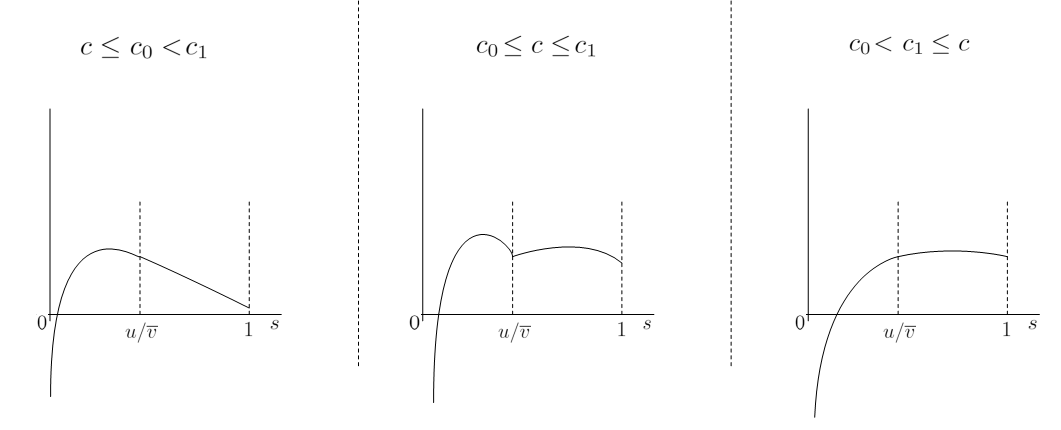
\includegraphics[scale=0.55]{Figure1}
\caption{Profits with regulator: interior solutions}\label{Figure1}}
\end{figure}


\begin{figure}[H]
\leftskip 1,5cm{
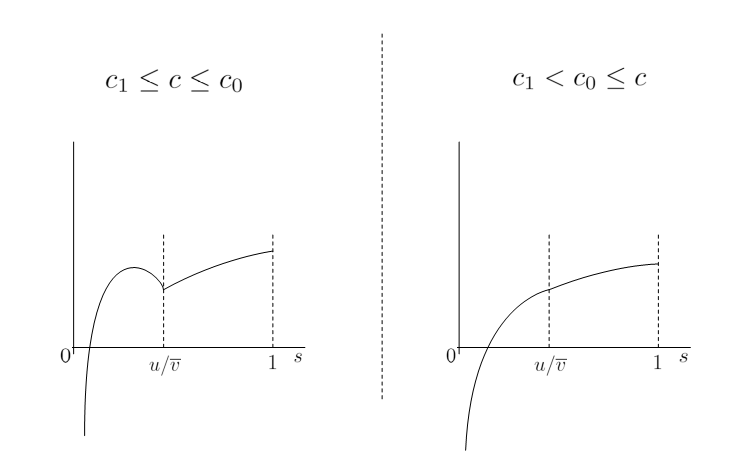
\includegraphics[scale=0.55]{Figure2}
\caption{Profits with regulator: corner solutions}\label{Figure2}}
\end{figure}

\medskip

The data processing cost is key to understand the effect of the regulator on information sharing. Low processing costs will make it less profitable to share more information, and firm 2 will optimally purchase $s\in[0,u/\ov]$. High processing costs will give incentives to firm 2 to purchase more, and will add a new effect to information sharing: in case the merger is declined, the higher the $s$ the higher the profits of firm 2 under competition.

\medskip

\subsubsection{Does the presence of the regulator drive up or down consumer information sharing?}

If $s\leq\frac{u}{\ov}$:

\begin{equation}
    \begin{aligned}
\pi_{2r}'(s^*)&=(1-\a)[a'(s^*)(\ov(1+s^*)-u)+(a(s^*)-1)\ov]< 0
    \end{aligned}
\end{equation}

Thus if there is a maximum on $[0,u/\ov]$, the optimal amount of data shared is smaller than without a regulator.

\bigskip

If $s\geq\frac{u}{\ov}$:

\begin{equation}
    \begin{aligned}
\pi_{2r}'(s^*)&=(1-\a)[a'(s^*)(\ov(1-s^*)+u)+(1-a(s^*))\ov]\\
            &=(1-\a)(-(\ov(1-s^*)+u)\frac{\ov u}{(\ov(1-s^*)+2u)^2}+\frac{\ov u}{(\ov(1-s^*)+2u)})\\
            &=(1-\a)\frac{\ov u^2}{(\ov(1-s^*)+2u)^2}\geq0\\
\end{aligned}
\end{equation}

\medskip

In this case, firm 2 purchases \textit{more} information from firm 1 than without the regulator. 

To sum up there are two cases to consider: if $s\leq u/ \ov$, more information sharing decreases the exploitation costs but lowers the probability that the merger is accepted.

\medskip

If $s\geq u/ \ov$ there is an additional positive effect of information sharing on the profits of firm 2: if the merger is prevented, the larger the $s$, the higher the profits of firm 2 under competition. With uniform distribution we can show that this second effect dominates the first one on $[u/\ov,1]$, and firm 2 purchases more information than without a regulator. 

\begin{prop}~~

\begin{itemize}
    \item When $s^*\in[0,u/\ov]$ the presence of the regulator reduces the amount  of information shared in equilibrium.
    \item When $s^*\in[u/\ov,1]$ the presence of the regulator increases the amount  of information shared in equilibrium.
\end{itemize}

\end{prop}


\subsubsection{The impact of the regulator on consumer surplus.}

Without regulator, when firm 2 purchases $s^*$ of information, the expected consumer surplus is:

\[
\a\uv s^*
\]

Clearly consumer surplus surplus increases with $s^*$, as consumers benefit from higher competition between firms in case synergies are low and the merger does not occurs.

\medskip

With the presence of a regulator, does firm 2 find it profitable to purchase $s$ data?

Yes if $\E[v]<u$ and

$$(1-\a)(\ov -u)-\a \uv s\geq c(s)$$

or if $\E[v]\geq u$ and

$$\a(u-\uv(1+s))\geq c(s)$$

With the presence of a regulator, does firm 2 find it profitable to purchase $s$ data?

Yes if $\E[v]<u$ and

$$(1-\a)[a(s)\ov+(1-a(s))(\ov s-u)-\ov s]-\a\uv s-c(s)\geq 0$$

or 

$$(1-\a)[a(s)\ov+(1-a(s))(\ov s-u)-u)-\a\uv s-c(s)\geq 0$$

It is clear that the presence of the regulator can prevent firm 2 to purchase information while information sharing would be the optimal strategy without a regulator. In this case, the presence of the regulator harms consumers: as no information is shared, the expected surplus is $0<\a \uv s$.

\medskip

If firm 2 purchases $s\in[u/\ov,1]$ data, $s>s^*$ and consumer surplus is equal to $\a \uv s+(1-a(s))u>\a \uv s^*$. In this case the presence of the regulator increases consumer surplus. 

\medskip

If firm 2 purchases $s\in[0,u/\ov]$ data, $s<s^*$ and consumer surplus is equal to $\a \uv s+(1-a(s))\ov s$. In this case the presence of the regulator has an ambiguous effect on consumer surplus. 


\medskip

\begin{prop}~~

\begin{itemize}
    \item When $s^*\in[0,u/\ov]$ the presence of the regulator has two opposite effects on consumer surplus:
    \begin{itemize}
        \item Less data is shared than without a regulator, which decreases consumer surplus.
        \item Mergers is prevented w.p. $1-a$, even when synergies are high, which increases consumer surplus.
    \end{itemize}
    \item When $s^*\in[u/\ov,1]$ the presence of the regulator always increases consumer surplus.
\end{itemize}

\end{prop}

\medskip

\subsection{Regulating pre-merger information sharing}

The regulator can allow or prevent firm 2 from purchasing information from firm 1 before sharing occurs. Before learning the value of $\rho$, the regulator compares social welfare with and without information sharing and chooses whether to allow firms to share.\footnote{The regulator does not know $\rho$ at the time of this decision for instance as $\rho$ be market specific and the decision to allow information sharing or not is for all markets. Moreover, if the regulator allows or prevents information sharing while knowing $\rho$, this would send a signal to firm 2 on the value of $\rho$.}

\medskip

Without information sharing, either $\E[v]<u$, firms do not merge and the expected gain in social welfare is equal to zero. Information sharing either allows the merger to proceed, and in this case the gain in social welfare is equal to $\rho (\ov-u)$. The merger is prevented if the social welfare is larger than with a merger, and $(1-\rho)\min{u,\ov s}+\rho (\max{u-\ov s,\ov s-u})\geq \rho \ov$.

\medskip

If $\E[v]\geq u$, either the merger is allowed, and social welfare is equal to $\rho \ov$, which is equal to welfare without information sharing. Or the merger is prevented because competition yields a larger welfare.

\medskip

Thus information sharing is always beneficial for the regulator, as when choosing to allow or prevent the merger, the regulator can always allow it and reach a social welfare equal to the case without information sharing. The regulator thus guarantees that social welfare is at least as good with information sharing as without, and information sharing allows the regulator to prevent merger when competition is more beneficial.


\begin{prop}~~

A regulator always has interest to allow firm to share information.

\end{prop}



\section{Bilateral information sharing}

We have focused on the case where firm 2 purchases information from firm 1. In practice firms can also engage in bilateral sharing of information, which we analyze in this section.\footnote{For instance \cite{scaria2018study} describes practices of information sharing between companies in Europe.} Bilateral information sharing is reminiscent of practices of cross licensing \citep{fershtman1992cross}.


\subsection{Competition}

Suppose now that firm $1$ shares $s_1\geq 0$ and firm 2 shares $s_2\geq0$, and let us ignore for the moment the possibility of a merger. If firm $2$ invests $c$ and learns $v$, it can provide its customers a value $vs_1$. Again we assume that only firm 2 chooses whether to invest $c(s_1)$, and after the investment is made, both firms learn the synergy. In this case, firm $1$ also learns $v$ and it can provide its customers a value $u+\beta v s_2$. Assuming Bertrand competition, it follows that the equilibrium price paid by the consumers and the profit per consumer are

\begin{align}
\begin{cases}
    p=v (s_1-\beta s_2)-u ; \pi_1(v,s_1,s_2)=0 ; \pi_2(v,s_1,s_2)=v(s_1-\beta s_2)-u & \text{ if }v (s_1-\beta s_2)\geq u\\ 
    p=u-v (s_1-\beta s_2) ; \pi_1(v,s_1,s_2)=u-v(s_1-\beta s_2); \pi_2(v,s_1,s_2)=0 & \text{ if }v (s_1-\beta s_2)\leq u.
\end{cases}
\end{align}


\subsection{Profits with data sharing}

Suppose firm $1$ shares $s_1$ with firm $2$, and that firm $2$ shares $s_2$ with firm $1$ in exchange of $s_1$. 

Upon receiving $s_1$ and $s_2$, Firm 2 can decide to invest $c(s)$ in order to learn $v$. In this case, the two firms anticipate payoffs $\pi_i(v, s_1,s_2)$ as given  Eq. \eqref{compbil} if there is no merger. Firm $2$ can make a TIOLI offer to buy firm $1$'s asset at a price $p(v, s_1,s_2)$ that will make firm $1$ indifferent between merging and not merging, that is 
%
\begin{equation}
    p(v, s_1,s_2):=\pi_1(v, s_1,s_2).  
\end{equation}


If $\beta\leq 0$ data sharing by firm 2 reduces the profits of firm 1, which in turn has no incentives to share information. We consider $\beta\geq 0$ and we write $\delta s=s_1-\beta s_2\in [-\beta,1]$.

%
\begin{itemize}
    \item With probability $\a$, $v=\uv<u$:
\begin{itemize}
    \item If $\uv \delta s\leq u$:
\begin{itemize}
    \item $\pi_1(\uv,\delta s)=u-\uv \delta s$;
    \item $\pi_2(\uv,\delta s)=0$;
\end{itemize}    
    \item If $\uv \delta s\geq u$:
\begin{itemize}
    \item $\pi_1(\uv,\delta s)=0$;
    \item $\pi_2(\uv,\delta s)=\uv\delta s-u$;
\end{itemize}
\end{itemize}
    \item With probability $1-\a$, $v=\ov>u$:
\begin{itemize}
    \item If $\ov \delta s\leq u$:
\begin{itemize}
    \item $\pi_1(\ov,\delta s)=u-\ov \delta s$;
    \item $\pi_2(\ov,\delta s)=0$;
\end{itemize}    
    \item If $\ov \delta s\geq u$:
\begin{itemize}
    \item $\pi_1(\ov,\delta s)=0$;
    \item $\pi_2(\ov,\delta s)=\ov\delta s-u$;
\end{itemize}
\end{itemize}
\end{itemize}

In this case, the expected payoff of firm 1 from sharing $\delta s$ information is:

\begin{itemize}
    \item If $\delta s\leq u/\ov$:
    
    $$\pi_1(\delta s)=\a(u-\uv \delta s)+(1-\a)(u-\ov \delta s)$$
    
    and necessarily  firm 2 needs $\delta s\leq0$ so that firm 1 accepts to share information.
    \item If $u/\ov\leq \delta s\leq u/\uv$:
    $$\pi_1(\delta s)=(1-\a)(u-\ov \delta s)$$
    and $\delta s<0$, which is impossible as $\delta s\geq u/\ov$.
    \item If $u/\uv\leq \delta s$:
    $$\pi_1(\delta s)=0$$
    and $\delta s<0$, which is impossible as $\delta s\geq u/\uv$.
\end{itemize}

Thus in equilibrium, bilateral information sharing can occur if $\delta s\leq0$.

The expected payoff of firm $2$ of sharing $s_2$ and investing $c(s_1)$ following sharing of data and learning $v$ is:


        $$\pi_2(s_1,s_2)=(1-\a)(\ov-u+\ov (s_1-\beta s_2))-c(s_1).$$
with $s_2\geq s_1$

\medskip
\subsection{Information acquisition}

We analyze whether it is profitable for firm 2 to exchange bilateral information with firm 1, and we characterize the optimal information sharing. The alternative for firm 2 is to purchase data and make profits as described in Section \ref{infacq}. We show that bilateral sharing can dominate information purchasing for firm $2$. 

\medskip

It is clear that $\pi_2(s_1,s_2)$ is maximized for the highest $s_1$ under the condition that $s_1\leq \beta s_2$. 


If $\beta\leq 1$, $s_2=1$, $s_1=\beta$ and

        $$\pi_2(s_1,s_2)=(1-\a)(\ov-u)-c(\beta).$$

If $\beta\geq 1$, $s_2=\frac{1}{\beta}$, $s_1=1$ and

        $$\pi_2(s_1,s_2)=(1-\a)(\ov-u).$$

\medskip

Let's compare profits in equilibrium under bilateral information sharing and information purchasing:

$$\pi_2(s^*)=(1-\a)(\ov-u)-2\sqrt{c\a \uv}+c.$$

where $-2\sqrt{c\a \uv}+c<\sqrt{c\a \uv}$ as $s^*=\sqrt{\frac{c}{\a\uv}}\leq 1$.

Bilateral sharing is always more profitable than information purchasing if $\beta\geq1$. Sharing information with firm 1 is a costless way to learn the synergies. In case synergies are low, no merger occurs and firm 2 has lost no money. In case synergies are high, firm 2 can acquire firm 1 at price $u$.

\medskip

If $\beta\leq1$, bilateral information sharing is more profitable than information purchasing iff $\sqrt{c}\leq 2\beta \sqrt{\a \uv}$. Thatis, if $\beta\geq\beta_0=\sqrt{\frac{c}{4\a \uv}}$.

\medskip

%
Similarly to information purchasing, there are two opposite effects of bilateral information sharing on the profits of firm 2. On the one hand, bilateral information sharing allows firm 2 to incentivize firm 1 to share information without money transfer. In turn, the higher $s_1$ the lower the data exploitation cost and the higher the benefits of firm 2 from avoiding low efficiency mergers. On the other hand, $s_2$ must be large enough to cover the loss of firm 1 due to competition in case merger does not occur, which increases the price firm 2 has to pay to acquire firm 1. 

\medskip

This leads us to the following proposition:

\begin{prop}~~

Bilateral information sharing yields higher profits than information purchasing if the information shared by firm 2 is profitable enough for firm 1, i.e., if $\beta\geq\beta_0$.

If $\beta\geq 1$, bilateral information sharing yields the same profits for firm 2 as if there was no information asymmetry at the beginning of the game.

\end{prop}

\medskip

\subsection{Social welfare}

\medskip

We compare social welfare under information purchasing with welfare under bilateral information sharing. For simplicity we focus on $\beta\geq1$, and bilateral information sharing is always more profitable for firm 2 and yields the highest possible outcome.

\medskip

If $v=\uv$ firm 2 does not acquire firm 1 and social welfare is equal to:

\[
(1-\rho) u+\uv \rho
\]

with bilateral information sharing, and to

\[
(1-\rho) (u-\uv s^*)+\uv s^*\rho
\]

with information purchasing.

\medskip

If $v=\ov$ firm 2 tries to acquire firm 1. If the merger is authorized, social welfare under bilateral information sharing is identical to information purchasing. If the merger is prevented, social welfare under bilateral sharing is equal to:

\medskip

\[
(1-\rho) u +\ov \rho
\]

\medskip

And welfare under information purchasing if $u\leq \ov s^*$ is equal to

\medskip

\[
(1-\rho) (\ov s^*-u)+u\rho
\]

\medskip

And whether bilateral information sharing yields higher welfare than information purchasing is ambiguous.

\medskip

If $u\geq \ov s^*$ 

\[
(1-\rho) (u-\ov s^*)+\ov s^*\rho
\]

And whether bilateral information sharing always yields higher welfare than information purchasing.


\medskip

\begin{prop}~~

If $v=\ov$ and $u\leq \ov s^*$, bilateral information sharing can lead to higher or lower welfare than information purchasing. 

Else, bilateral information sharing always leads to higher welfare than information purchasing.

\end{prop}

\medskip

The fact than in general, bilateral information sharing yields higher profits than information purchasing results from two effects. First, as firm 2 shares information, more information on the markets increases firm competition and consumer surplus. Secondly, as firm 2 shares information, firm 1 can enhance product quality and make higher profits. In equilibrium, the gains in profits for firm 1 from receiving $s_2$ cover its loss from sharing $s_1$. 

\medskip

\bibliographystyle{agsm}
\bibliography{biblio-synergies.bib}



\appendix

\section{Appendix A: proofs}

\section{Appendix B: extensions}


\subsection{Firm 2 privately learns synergies}

Consider now the situation where, after having acquired $s$ and invested, firm 2 learns $v$ privately. Firm 1 does not know $v$ and the payoffs are the following:


\begin{align}\label{compbilmixed}
\begin{cases}
    w.p.~~ \a,~~ \pi_1(s)=u-\uv s, \pi_2(s)=0\\ 
    w.p.~~ 1-\a,~~ \pi_1(s)=\max\{u-\ov s,0\}, \pi_2(s)=\max\{\ov s-u,0\}\\ 
\end{cases}
\end{align}

\paragraph{Pooling}

Regardless of the value of the synergy, firm 2 offers to acquire firm 1 at price $p(s)$:

\begin{align}
\begin{cases}
    IC:~~ p(s)\geq \a(u-\uv s)+\max\{u-\ov s,0\};\\ 
    IR_L:~~ \uv -p(s)\geq 0;\\
    IR_H:~~ \ov -p(s)\geq \ov s-u;\\ 
\end{cases}
\end{align}


Thus we have $\uv \geq p(s)$ and $\ov(1-s)+u\geq p(s)$ and $IR_L\implies IR_H$. Thus pooling is an equilibrium if and only if $\uv\geq \a(u-\uv s)+\max\{u-\ov s,0\}$. 

In this case, the expected payoff of firm 1 when sharing $s$ is $\a(u-\uv s)+\max\{u-\ov s,0\}$, and the price of information is $T(s)=u-\a(u-\uv s)-\max\{u-\ov s,0\}$. 

The expected payoff of firm 2 is then:

\[
\pi_2(s)=(1-\a) \ov +\a\uv -u-c(s)
\]


And there is no benefits from sharing information. 

If $\uv\leq \a(u-\uv s)+\max\{u-\ov s,0\}$ pooling cannot be an equilibrium. 


\paragraph{Excluding}

If $\uv\leq \a(u-\uv s)+\max\{u-\ov s,0\}$ pooling cannot be an equilibrium and firm 2 makes an offer only when $v=\ov$. 

\begin{align}
\begin{cases}
    IC:~~ p(s)\geq \a(u-\uv s)+\max\{u-\ov s,0\};\\ 
    IR_H:~~ \ov -p(s)\geq \ov s-u;\\ 
\end{cases}
\end{align}

The optimal price of acquisition is $p(s)=\a(u-\uv s)+\max\{u-\ov s,0\}$, and the expected payoff of firm 1 from selling $s$ information is $\a(u-\uv s)+\max\{u-\ov s,0\}$, and the price of information is $T(s)=u-\a(u-\uv s)-\max\{u-\ov s,0\}$.


The expected payoff of firm 2 is then:

\[
\pi_2(s)=(1-\a) \ov-u-c(s)
\]

and information sharing is less profitable than merger under imperfect information.



\paragraph{Separating:}

\medskip  

In a separating equilibrium firm 2 pays two different prices $\up$ when synergies are $\uv$ and $\op$ when synergies are $\ov$. It is clear that when synergies are low, firm 2 does not have interest to acquire firm 1 and separating equilibrium is not sustainable.

\medskip

\begin{prop}~~

Information sharing is never optimal when synergies are learned privately.

\end{prop}

It is thus essential that firm 1 learns the value of the synergy. It is also clear that the learning process must be transparent. Else, firm 2 may have interest to claim that synergies are high and to acquire firm 1 at a low cost.



\subsection{Bilateral information sharing 2}


We consider alternative profits for firm 1 from receiving information from firm 2.

\subsubsection{Competition}

Suppose now that firm $1$ shares $s_1\geq 0$ and firm 2 shares $s_2\geq0$, and let us ignore for the moment the possibility of a merger. If firm $2$ invests $c$ and learns $v$, it can provide its customers a value $vs_1$. Again we assume that only firm 2 chooses whether to invest $c(s_1)$, and after the investment is made, both firms learn the synergy. In this case, firm $1$ also learns $v$ and it can provide its customers a value $max\{u,vs_2\}$ (taking the maximum allows to avoid destructive synergies due to reputation effects that do not arise when firms compete). Assuming Bertrand competition, it follows that the equilibrium price paid by the consumers and the profit per consumer are

\begin{align}\label{compbil}
\begin{cases}
    p=v s_1-\max\{u,v s_2\}; \pi_1(v,s_1,s_2)=0; \pi_2(v,s_1,s_2)=v s_1-\max\{u,v s_2\} & \text{ if }v s_1\geq \max\{u,v s_1\}\\ 
    p=\max\{u,v s_2\}-v s_1; \pi_1(v,s_1,s_2)=\max\{u,v s_2\}-v s_1; \pi_2(v,s_1,s_2)=0 & \text{ if }v s_1\leq \max\{u,v s_2\}.
\end{cases}
\end{align}


\subsubsection{Profits with data sharing}

Suppose firm $1$ shares $s_1$ with firm $2$, and that firm $2$ shares $s_2$ with firm $1$ in exchange of $s_1$. 

Upon receiving $s_1$ and $s_2$, Firm 2 can decide to invest $c(s)$ in order to learn $v$. In this case, the two firms anticipate payoffs $\pi_i(v, s_1,s_2)$ as given  Eq. \eqref{compbil} if there is no merger. Firm $2$ can make a TIOLI offer to buy firm $1$'s asset at a price $p(v, s_1,s_2)$ that will make firm $1$ indifferent between merging and not merging, that is 
%
\begin{equation}\label{merger-pricebil}
    p(v, s_1,s_2):=\pi_1(v, s_1,s_2).  
\end{equation}


If $s_2\leq \frac{u}{\ov}$ data sharing by firm 2 does not impact the profits of firm 1, which in turn has no incentives to share information. We consider $s_2\geq \frac{u}{\ov}$ and we write $\delta s=s_1-s_2\in [-1,1-\frac{u}{\ov}]$.

%
\begin{itemize}
    \item With probability $\a$, $v=\uv<u$:
\begin{itemize}
    \item $\pi_1(\uv,s_1)=u-\uv s_1$;
    \item $\pi_2(\uv,s_1)=0$;
\end{itemize}
    \item With probability $1-\a$, $v=\ov>u$:
\begin{itemize}
    \item If $ s_1\leq s_2$, $\delta s\leq 0$ and:
\begin{itemize}
    \item $\pi_1(\ov,\delta s)=-\ov \delta s$;
    \item $\pi_2(\ov,\delta s)=0$;
\end{itemize}    
    \item If $s_1\geq s_2$, $\delta s\geq 0$ and:
\begin{itemize}
    \item $\pi_1(\ov,s)=0$;
    \item $\pi_2(\ov,s)=\ov \delta s$;
\end{itemize}
\end{itemize}
\end{itemize}

In this case, the expected payoff of firm 1 from sharing $\delta s$ information is:

\begin{itemize}
    \item If $\delta s\leq 0$, firm 2 pays a positive price to firm 1 for the merger when $v=\ov$:
    $$\pi_1(s)=\a(u-\uv s_1)+(1-\a)(-\ov \delta s)$$
    
    and $(1-\a)\ov s_2 \geq (1-\a)u+\E[v]s_1$
    \item If $\delta s\geq 0$, firm 2 acquires firm 1 for a zero price:
    $$\pi_1(s)=\a(u-\uv s_1)$$
    and $s_1=-\frac{1-\a}{\a}\frac{u}{\uv}$, which is impossible as $s_1 \geq 0$.
\end{itemize}

Thus in equilibrium, bilateral information sharing can occur if $\delta s\leq0$, and in this case $(1-\a)\ov s_2 = (1-\a)u+\E[v]s_1$.

The expected payoff of firm $2$ of sharing $s_2$ and investing $c(s_1)$ following sharing of data and learning $v$ is:

\begin{equation}
    \begin{aligned}
    \pi_2(s_1,s_2)=&(1-\a)\ov(1-s_2+s_1)-c(s_1)\\
                =&(1-\a)\ov-(1-\a)u-\a \uv s_1-c(s_1)
    \end{aligned}
\end{equation}


with $s_2\geq s_1$

\medskip

\subsubsection{Information acquisition}

We analyze whether it is profitable for firm 2 to exchange bilateral information with firm 1, and we characterize the optimal information sharing. The alternative for firm 2 is to purchase data and make profits as described in Section \ref{infacq}. We show that bilateral sharing can be equivalent to information purchasing for firm $2$. 

\medskip

It is clear that $\pi_2(s)$ is maximized for $s_1$ such that 

$$\a \uv =-c'(s_1^*)$$

under the condition that $(1-\a)\ov s_2 \geq (1-\a)u+\E[v]s_1$. Thus in equilibrium, 

\medskip

Bilateral sharing is more profitable than information purchasing if:

$$(1-\a)(\ov-u)-\a\uv s_1^* -c(s_1^*)\geq(1-\a)(\ov -u)-\a \uv s^*-c(s^*).$$

\medskip

As $s_1^*$ is chosen under constraints, either $s_1^*=s^*$ and information purchasing is equivalent to bilateral information sharing, or $s_1^*< s^*$ and information purchasing yields higher profits than information sharing. 

\medskip
%
Similarly to information purchasing, there are two opposite effects of bilateral information sharing on the profits of firm 2. On the one hand, bilateral information sharing allows firm 2 to incentivize firm 1 to share information without money transfer. In turn, the higher $s_1$ the lower the data exploitation cost and the higher the benefits of firm 2 from avoiding low efficiency mergers. On the other hand, $s_2$ must be large enough to cover the loss of firm 1 due to competition in case merger does not occur, which increases the price firm 2 has to pay to acquire firm 1. 

\medskip

This leads us to the following proposition:

\begin{prop}~~\label{prop:1bil3}


\begin{itemize}
    \item Information purchasing is always at least as good as bilateral information sharing.  
    \item Bilateral information sharing is equivalent to information purchasing when $s_1^*=s^*$.
    \item Bilateral information sharing can be optimal when information purchasing is prevented.
\end{itemize}

\end{prop}

\medskip

\subsubsection{Social welfare}

\medskip

We compare social welfare under information purchasing with welfare under bilateral information sharing. 

\medskip

If $v=\uv$ firm 2 does not acquire firm 1 and social welfare is equal to:

\[
(1-\rho) (u-\uv s_1^*)+\uv s_1^*\rho
\]

\medskip

If $\rho\in[0,1/2]$, welfare is higher under the regime that yields the lowest $s_1$, that is, under bilateral information sharing. If $\rho\in[1/2,1]$ the opposite is true.

\medskip

If $v=\ov$ firm 2 tries to acquire firm 1. If the merger is authorized, social welfare under bilateral information sharing is identical to information purchasing. If the merger is prevented, social welfare under bilateral sharing is equal to:

\medskip

\[
(1-\rho) \ov (1-s_1^*)+\ov s_1^*\rho
\]

\medskip

And welfare under information purchasing if $u\leq \ov s^*$ is equal to

\medskip

\[
(1-\rho) (\ov (1-s^*)+u)+u\rho
\]

\medskip

If $u\geq \ov s^*$ 

\[
(1-\rho) (\ov (1+s^*)-u)+\ov s^*\rho
\]

\medskip

\begin{prop}~~


\end{prop}

\medskip

\subsection{Mixed strategy: bilateral information sharing \& information purchasing}

Firm 2 can now both purchase information from firm 1 and share some of its own information at the same time. The competition stage is identical to the previous section and we directly go to profit functions and the price of information under mixed strategies. 

\medskip

\subsubsection{Profits with data sharing}

Suppose firm $1$ shares $s_1$ with firm $2$, and that firm $2$ shares $s_2$ with firm $1$ in exchange of $s_1$. 

Upon receiving $s_1$, firm 2 can decide to invest $c(s_1)$ in order to learn $v$. In this case, the two firms anticipate payoffs $\pi_i(v,s_1,s_2)$ as given by Eq. \eqref{compbil} if there is no merger. Firm $2$ can make a TIOLI offer to buy firm $1$'s asset at a price $p(v,s_1,s_2)$ that will make firm $1$ indifferent between merging and not merging, that is 
%
\begin{equation}\label{merger-pricebil2}
    p(v,s_1,s_2):=\pi_1(v,s_1,s_2).  
\end{equation}
%

\begin{itemize}
    \item With probability $\a$, $v=\uv<u$:
\begin{itemize}
    \item $\pi_1(\uv,s_1)=u-\uv s_1$;
    \item $\pi_2(\uv,s_1)=0$;
\end{itemize}
    \item With probability $1-\a$, $v=\ov>u$:
\begin{itemize}
    \item If $ s_1\leq s_2$, $\delta s\leq 0$ and:
\begin{itemize}
    \item $\pi_1(\ov,\delta s)=-\ov \delta s$;
    \item $\pi_2(\ov,\delta s)=0$;
\end{itemize}    
    \item If $s_1\geq s_2$, $\delta s\geq 0$ and:
\begin{itemize}
    \item $\pi_1(\ov,s)=0$;
    \item $\pi_2(\ov,s)=\ov \delta s$;
\end{itemize}
\end{itemize}
\end{itemize}

In this case, the expected payoff of firm 1 from sharing $\delta s$ information is:

\begin{itemize}
    \item If $\delta s\leq 0$, firm 2 pays a positive price to firm 1 for the merger when $v=\ov$:
    $$\pi_1(s_1,s_2)=\a(u-\uv s_1)+(1-\a)(-\ov \delta s)+T(s_1,s_2)$$
    
    and $(1-\a)\ov s_2+T(s_1,s_2) \geq (1-\a)u+\E[v]s_1$
    \item If $\delta s\geq 0$, firm 2 acquires firm 1 for a zero price:
    $$\pi_1(s_1,s_2)=\a(u-\uv s_1)+T(s_1,s_2)$$
    and $T(s_1,s_2)=(1-\a)u+\a \uv s_1$.
\end{itemize}


If $\delta s\leq 0$:

\begin{equation}
    \begin{aligned}
      \pi_2(s_1,s_2)&=(1-\a)(\ov(1+\delta s))-c(s_1)-T(s_1,s_2)\\
                    &=(1-\a)(\ov(1+\delta s))-c(s_1)+(1-\a)\ov s_2-(1-\a)u-\E[v]s_1\\
                    &=(1-\a)(\ov-u)-c(s_1)-\a\uv s_1\\
    \end{aligned}
\end{equation}


If $\delta s\geq 0$:

\begin{equation}
    \begin{aligned}
      \pi_2(s_1,s_2)&=(1-\a)\ov-c(s_1)-T(s_1,s_2)\\
                    &=(1-\a)\ov-c(s_1)-(1-\a)u-\a \uv s_1\\
                    &=(1-\a)(\ov-u)-c(s_1)-\a\uv s_1\\
    \end{aligned}
\end{equation}

\subsubsection{Optimal information acquisition}


\medskip

\begin{equation}
    \begin{aligned}
      \pi_2(s_1,s_2)&=(1-\a)(\ov-u)-c(s_1)-\a \uv s_1\\
      \frac{\partial\pi_2(s_1,s_2)}{\partial s_1}&=-c'(s_1)-\a \uv \\
    \end{aligned}
\end{equation}

And the optimal amount of information shared by firm 1 is identical to information purchasing. 

\medskip


\end{document}
